\section{Stand der Forschung} \label{SdF}

Bevor auf den Stand der Forschung mit den Technologien und Konzepten zur Energieeinsparung eingegangen wird, soll im Folgenden auf relevante Begrifflichkeiten eingegangen werden. Die Begrifflichkeiten sollen zunächst definiert und im Anschluss für die Arbeit abgegrenzt werden.  

\subsection{Begriffe}

\subsubsection{Wirtschaftlichkeit}
  Bei der Betrachtung von Energieeinsparpotentialen in Netzwerken findet die Wirtschaftlichkeit häufig keine Beachtung. Die Wirtschaftlichkeit drück aus, wie sparsam mit vorhandenen Ressourcen umgegangen wurde.  Vor jeder Investition steht die Frage nach der betriebswirtschaftlichen Sinnhaftigkeit. Im ökonomischen Sinn bedeutet Wirtschaftlichkeit das Verhältnis aus monetären Kosten und Leistung. 

%TODO Hier fehlt noch etwas - Input Max

Für die Wirtschaftlichkeitsbetrachtung des Netzwerks werden die Ausgaben für die Anschaffung der Netzwerkkomponenten (Capex –- Capital Expenditures) nicht berück\-sichtigt. Die für den operativen Geschäftsbetrieb anfallenden Aufwendungen werden „Operating Expenditures“ (kurz Opex) genannt und stellen die Betriebskosten dar. Zu den laufenden Ausgaben für den Geschäfts\-betrieb gehören u.a. Mieten, Personal- und Energiekosten, Aufwendungen für Wartung und Support, Verbrauchsmaterialien und Betriebsstoffe. 

\subsubsection{Effizienz im Bereich von Telekommunikationsnetzen}
%TODO Hier fehlt noch etwas - Input Max

%Energieverbrauch im Verhältnis zur Datenmenge

%Energieeffizienz-Formeln beschreibt Alecsic in folgendem Artikel: https://onedrive.live.com/view.aspx?resid=E1D79E6BE5C4A7E2!6662&app=OneNote&authkey=!ADxabmEazZueeyU


%S. Aleksic, „Energy-Efficient Communication Networks for Improved Global Energy Productivity”, Telecommunication Systems, Vol. 54, No. 2 , 2013, pp. 183-199.
\subsubsection{Carrier-Netzwerke}
Gegenstand der Projektarbeit bildet ein hinsichtlich der Energieeffizienz und Wirtschaftlichkeit zu optimierendes Carrier-Netzwerk.

Unter einem Carrier versteht man […] eine Gesellschaft, die mindestens drei Übertra\-gungs\-wege betreibt, die über eine Vermittlungsstelle miteinander verbunden sein müssen"' (s. \cite{carrier}). Ein Carrier-Netzwerk stellt somit physikalische Transportwege und -verfahren zur Verfügung und bildet die Grundlage für sogenannte Value Added Services von Providern, welche auf den Carrier-Diensten aufsetzen (vgl. \cite{fassnacht}) . "`Bei den TK-Transportwegen unterscheidet man leitergebundene Verbindungen auf der Basis von Kupferkabeln oder Lichtwellenleitern sowie Funkverbindungen wie Satellitenverbindungen, Richtfunkstrecken und Rundfunkverbindungen"' (s. \cite{fassnacht}).

Somit umfasst ein Carrier-Netzwerk neben dem nur das physikalische Backbone-Netz, sondern auch das Zugangs- und Aggregationsnetzwerk. Das Kernnetz eines Carriers kann durch ein vereinfachtes Drei-Schichten-Modell dargestellt werden, das sich nach den Protokollschichten für Glasfaser, Ethernet und Internet richtet. 



\subsection{Technologien und Konzepte zur Reduzierung des Energieverbrauchs in Telekommunikationsnetzwerken}
Der aktuelle Stand der Forschung vermittelt Technologien und Entwicklungen, welche die zuvor genannten Konzepte umsetzen. Die im Folgenden genannten Technologien beziehen sich im Einzelnen auf eines der im vorherigen Kapitel genannten Konzepte. Bezüglich des reinen Telekommunikationsnetzes können Möglichkeiten zur Steigerung der Energieeffizienz bzw. Reduzierung des Energieverbrauchs wie folgt unterteilt werden:

\subsubsection{Energieeffiziente Netzelemente}
Durch den technologischen Fortschritt können Netzwerkkomponenten energieeffizienter gestaltet werden, beispielsweise durchzunehmende Integration mehrerer einzelner Geräte\-einheiten in einem Verbundgerät. Somit können mehrere Module in einer Einheit zusammengefasst werden ohne die Netzwerkarchitektur zu verändern. Betrachtet man einzelne Geräte kann durch den Austausch alter Hardware mit neueren, energieeffizienteren Komponenten eine Einsparung erzielt werden. 

\subsubsection{Energieeffiziente Netzarchitektur}
Ein Ansatz bezieht sich auf das Konzept der energieeffizienten Netzwerkarchitektur und sieht eine Vereinfachung des Netzes vor, welche durch eine geographische Aufteilung des Netzes in Submodale (Global - Kontinental - National - Regional - Zugang) erfolgen kann \cite{aleksic2014}. Durch das Einteilen in Submodale und Einsetzen von adäquaten Übertragungs\-technologien innerhalb der Abgrenzungen können die Einsparpotentiale unabhängig voneinander betrachtet werden.

\subsubsection{Verkehrslastadaptiver Netzbetrieb}

Durch den in der Einleitung erwähnten zunehmen Datenverkehr und dem daraus resultierenden Netzausbau führt eine nahezu konstante Leistungsaufnahme der Netzelemente zu einem Anstieg des Netzenergiebedarfs. Da jedoch die Verkehrslast des Netzes zeitlich variiert, können in Phasen geringerer Last einzelne Systeme in einem Modus mit niedrigerer Leistungsaufnahme betrieben werden, ohne dass eine Beeinträchtigung für die Nutzer entsteht.

Heutige Telekommunikationsnetze werden auf Basis einer Spitzenlast zuzüglich einer Reserve dimensioniert. Für die Dimensionierung der Netze stellt eine dynamische Anpassung der Netzkapazität an die Verkehrslast eine attraktive Lösung dar. %TODO QUELLE

Tageszeitabhängige Schwankungen der Netzauslastung ermöglichen eine unabhängige und dynamische Abschaltung von Ports und Links unter der Berücksichtigung der Quality of Service-Bedingungen \cite{aleksic2013}. Dabei werden Algorithmen zur Identifikation von individuell abschaltbaren Links verwendet \cite{fassnacht}. Die Verfasser W. Fisher, M. Suchara und J. Rexford schreiben in ihrer Veröffentlichung „Greening Backbone Networks: [...]“, dass die durchschnittliche Verbindungsauslastung der Backbone-Netzwerke vieler großer Internet Service Provider geschätzt 30-40\% betrage (vgl. \cite{fisher} S. 1). Abbildung \ref{fig:Netzdimensionierung} zeigt die beiden Prinzipien der Netzdimensionierung.

\begin{figure}[!ht]
	\centering
	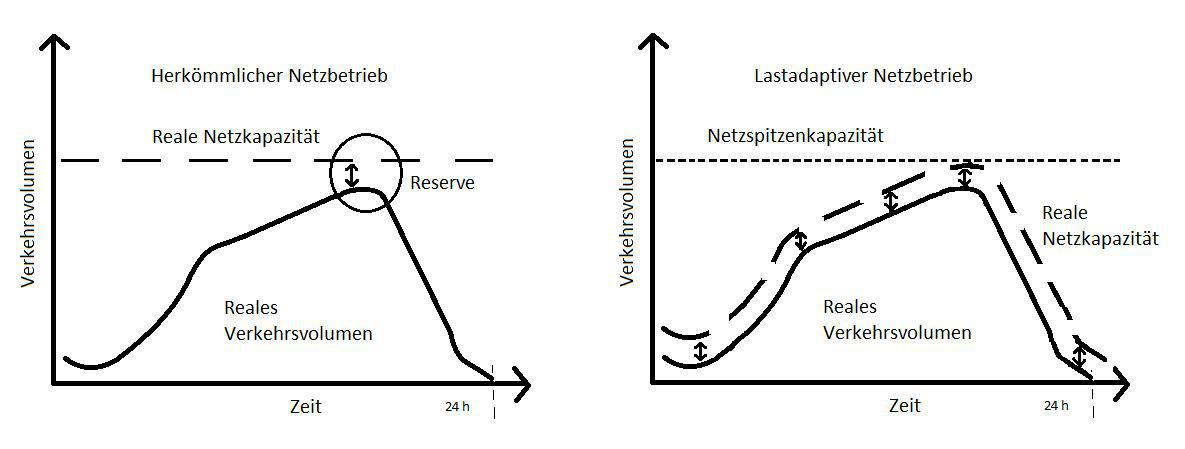
\includegraphics[width=0.8\textwidth]{Netzdimensionierung}
	\caption{Prinzipien der Netzdimensionierung}
	\label{fig:Netzdimensionierung}
\end{figure}

Der linke Teil der Abbildung zeigt Verkehrsvolumen in einem Netz, dessen Kapazität aufgrund einer Spitzenlast zuzüglich einer Reserve dimensioniert wurde. Es ist erkennbar, dass die reale Netzkapazität im Laufe eines Tages nur einmal annähernd erreicht wird. Je geringer der Abstand zwischen der Gerade der realen Netzkapazität und dem Graphen ist, desto effizienter ist das Netz. Durch die statische Netzkapazität ist ein konstanter Energieaufwand notwendig, um das Netz zu betreiben. Im rechten Teil der Abbildung ist dargestellt, wie durch den lastadaptiven Netzbetrieb ein effizienteres Netz gestaltet werden kann. Die reale Netzkapazität passt sich dem realen Verkehrsvolumen an und dessen Verläufe sind bis auf eine vorgehaltene Reserve gleich. Betrachtet man beide Teile der Grafik ist zu erkennen, dass der Abstand der Gerade und dem Graphen beim lastadaptiven Netzbetrieb um einige Vielfache geringer ist als bei dem statisch dimensionierten Netz. Somit ist das Netz um einige Vielfache effizienter.

Durch die Abschaltung einzelner Ports kann laut der Deutschen Telekom AG der Energiebedarf einiger Elemente um ein Drittel gesenkt werden (vgl \cite{lange} S. 4). Demnach verbrauchen Ports die, keinen Verkehr leiten signifikant weniger Energie als solche unter Last. Weiterhin wird beschrieben, dass durch die Deaktivierung ganzer Line Cards und Port Groups per Management Systems nahezu 100\% Einsparung erreicht werden kann. In dem Text von 2010 wird beschrieben, dass das Deaktivieren der Line Cards nur per manuellen Eingriff mit einem Network Management System erfolgen kann [.... C.Lange]. Der Aufwand für das dynamische, temporäre Abschalten steht nicht im Verhältnis zur Einsparung. Die Hersteller der Backbone-Netzwerk-Komponenten implementieren derzeit Funktionen, die das manuelle Eingreifen durch eine automatische Kapazitätsanpassung ersetzen. Die Herausforderung in den nächsten Jahren wird zum einen sein die Deaktivierungs- und Aktivierungszeiten der Elemente zu reduzieren. Weiterhin ist es notwendig die Betriebssysteme großer Router Systeme für die genannte Dynamik kompatibel zu machen, da aktuelle Softwarelösungen eine temporäre Aus- und Abschaltung nicht vorsehen.

\subsubsection{Hybrid Optical Swiching}
Optische leitungsvermittelnde Switche basieren auf mikro-elektromechanischen Systemen, die eine geringe Menge an Energie benötigen und eine hohe Portanzahl besitzen. Das sog. Hybrid Optical Switching (HOS) verwendet eine Kombination aus optischen und elektronischen Netzknoten. Zum einen wird „Optical Circuit Switching“ (OCS) verwendet, das laut C. Xin, C. Qiao, Y. Ye und S. Dixit in der Veröffentlichung „A Hybrid Optical Switching Approach“ als fortgeschrittene und viel verwendete Technologie zur Übermittlung in optischen Netzwerken eingesetzt wird. OCS ist gut geeignet für langanhaltende und kontinuierliche Datenströme, jedoch kommt die Technik bei stoßweisen Anstieg des Durchsatzes an ihre Grenzen. Eine alternative Technologie stellt „Optical Burst Switching“ (OBS) dar. Wie der Name darlegt ist die Technologie optimiert für kurzzeitig, ansteigende Datendurchsätze. Ein Nachteil der Technik ist die abnehme Leistung bei lang andauernden, kontinuierlichen Strömen. Weiterhin stellt OBS eine hohe Bandbreitennutzung her, benötigt hierfür aber große optische Pufferspeicher. Um effektiv beide Varianten der Datenströme zu übertragen, können mit der Kombination von OCS und OBS die Vorteile beider Technologien erreicht werden. Die beiden Technologien sind als komplementäre Ansätze anzusehen. [Xin, C. Qiao, Y. Ye und S. Dixit]. In einem HOS-Netzwerk werden große Datenströme durch vorgehalten Leitungen oder mit langen Durchsatzstöße übertragen und kleinere Ströme durch einzelne Datenpakete und kurze Durchsatzstöße übermittelt.

\subsubsection{Adaptive Optical Swiching}

%TODO Max
%http://publik.tuwien.ac.at/files/PubDat_213899.pdf